\documentclass[tikz, border=12pt]{standalone}
\usepackage{tikz}
\usepackage{amsmath}

\begin{document}

% n=6 elements => 7 nodes => 7 hat functions
% h = 1.5cm spacing, hat height = 1.8cm
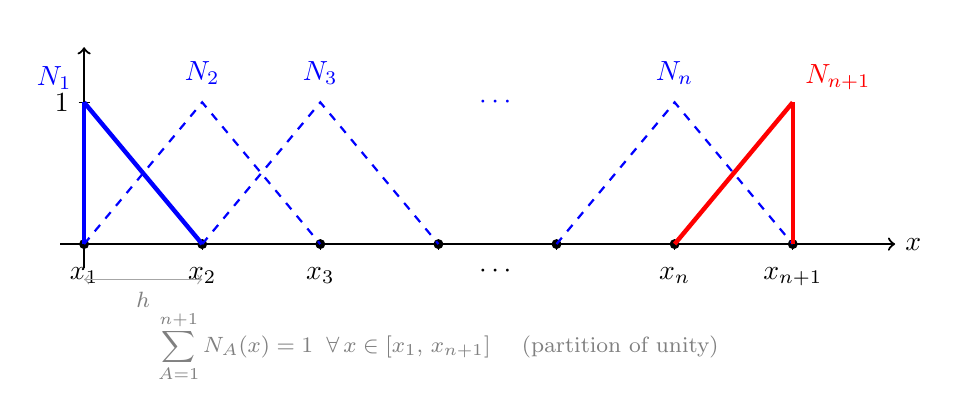
\begin{tikzpicture}[scale=1.0]

  % Spacing and height as lengths
  \def\h{1.5}   % node spacing (cm)
  \def\hh{1.8}  % hat peak height (cm)

  % Horizontal axis
  \draw[->, thick] (-0.3, 0) -- (10.3, 0) node[right] {$x$};

  % Vertical axis
  \draw[->, thick] (0, -0.3) -- (0, 2.5) node[above] {};

  % Tick at 1 on vertical axis
  \draw[thin] (-0.07,\hh) -- (0.07,\hh) node[left=4pt] {$1$};

  % Node positions: x_A = (A-1)*h, A=1..7
  % x1=0, x2=1.5, x3=3.0, x4=4.5, x5=6.0, x6=7.5, x7=9.0

  % Node dots and x-axis ticks
  \foreach \xpos/\lbl in {
    0/{x_1},
    1.5/{x_2},
    3.0/{x_3},
    4.5/{},
    6.0/{},
    7.5/{x_n},
    9.0/{x_{n+1}}
  }{
    \fill (\xpos, 0) circle (1.8pt);
    \draw[thin] (\xpos,-0.07)--(\xpos,0.07);
    \ifx\lbl\empty
    \else
      \node[below=5pt] at (\xpos,0) {$\lbl$};
    \fi
  }

  % Ellipsis between x3 and xn on the axis
  \node at (5.25, -0.35) {$\cdots$};

  % Element length annotation — placed just below the axis tick labels
  \draw[<->, thin, gray!70] (0,-0.45) -- (1.5,-0.45);
  \node[gray, below=1pt] at (0.75,-0.45) {\footnotesize $h$};

  % ===========================================================
  % N_1: left boundary half-hat — solid blue
  % peak at x=0, drops to 0 at x=1.5
  % ===========================================================
  \draw[blue, ultra thick]
    (0, \hh) -- (1.5, 0);
  \draw[blue, ultra thick] (0,0) -- (0,\hh);
  \node[blue, above left=1pt] at (0,\hh) {$N_1$};

  % ===========================================================
  % N_2: full hat, dashed blue
  % peak at x=1.5
  % ===========================================================
  \draw[blue, thick, dashed]
    (0,0) -- (1.5,\hh) -- (3.0,0);
  \node[blue, above=3pt] at (1.5,\hh) {$N_2$};

  % ===========================================================
  % N_3: full hat, dashed blue
  % peak at x=3.0
  % ===========================================================
  \draw[blue, thick, dashed]
    (1.5,0) -- (3.0,\hh) -- (4.5,0);
  \node[blue, above=3pt] at (3.0,\hh) {$N_3$};

  % Indicate skipped interior basis functions
  \node[blue] at (5.25, \hh) {$\cdots$};

  % ===========================================================
  % N_n: full hat, dashed blue
  % peak at x=7.5 (second to last node)
  % ===========================================================
  \draw[blue, thick, dashed]
    (6.0,0) -- (7.5,\hh) -- (9.0,0);
  \node[blue, above=3pt] at (7.5,\hh) {$N_n$};

  % ===========================================================
  % N_{n+1}: right boundary half-hat — solid red
  % rises from 0 at x=7.5 to peak at x=9.0
  % ===========================================================
  \draw[red, ultra thick]
    (7.5, 0) -- (9.0, \hh);
  \draw[red, ultra thick] (9.0,0) -- (9.0,\hh);
  \node[red, above right=1pt] at (9.0,\hh) {$N_{n+1}$};

  % ===========================================================
  % Partition of unity note
  % ===========================================================
  \node[gray, align=center] at (4.5, -1.3)
    {\footnotesize
      $\displaystyle\sum_{A=1}^{n+1} N_A(x) = 1
      \;\;\forall\,x \in [x_1,\,x_{n+1}]$
      \quad (partition of unity)};

\end{tikzpicture}
\end{document}
